\documentclass[conference]{IEEEtran}
\IEEEoverridecommandlockouts
% The preceding line is only needed to identify funding in the first footnote. If that is unneeded, please comment it out.
\usepackage{cite}
\usepackage{amsmath,amssymb,amsfonts}
%\usepackage{algorithmic}
\usepackage{graphicx}
\usepackage{textcomp}
\usepackage{xcolor}
\usepackage{algorithmicx}
%\usepackage[colorlinks=true, allcolors=blue]{hyperref}
\usepackage{algpseudocode}
\usepackage{algorithm}
\usepackage{xspace}
\usepackage{hyperref}
\usepackage{numprint}
\usepackage{todonotes}

\def\BibTeX{{\rm B\kern-.05em{\sc i\kern-.025em b}\kern-.08em
T\kern-.1667em\lower.7ex\hbox{E}\kern-.125emX}}
% user-specified commands
%\newcommand{\R}{\mathbb{R}}
\newcommand{\N}{\mathbb{N}}
%\newcommand{\llminimal}{${\|\cdot\|}_2$-minimal\xspace}
\newcommand{\Pro}[1]{\mathbf{Pr} \left[\,#1\,\right]}
\newcommand{\pro}[1]{\mathbf{Pr} [\,#1\,]}
\newcommand{\Ex}[1]{\mathbb{E} \left[\,#1\,\right]}
\newcommand{\ex}[1]{\mathbb{E} [\,#1\,]}
\newcommand{\hit}{- [\pi]_s (H[v,s]-H[u,s])}

\newcommand{\Oh}{\ensuremath{\mathcal{O}}}


\newcommand{\centre}[1]{z_{#1}}
\newcommand{\centres}{Z}
\newcommand{\degree}{\operatorname{deg}}
\newcommand{\maxdeg}{\operatorname{maxdeg}}
\newcommand{\diam}{\operatorname{diam}}
\newcommand{\res}{\operatorname{res}}
\newcommand{\Res}{\operatorname{Res}}
%\newcommand{\cond}{\operatorname{cond}}
\newcommand{\Cond}{\operatorname{Cond}}
\newcommand{\proxy}{\operatorname{proxy}}
\newcommand{\excond}{\operatorname{ex\_cond}}
\newcommand{\exres}{\operatorname{ex\_res}}
\newcommand{\exalg}{\operatorname{ex\_alg}}
\newcommand{\dist}{\operatorname{dist}}
\newcommand{\cost}{\operatorname{c}}
\newcommand{\ord}{\operatorname{ord}}
\newcommand{\Vor}{\operatorname{Vor}}
\newcommand{\M}{\mathbf{M}}
\newcommand{\LL}{\mathbf{L}}
%\newcommand{\L}{\mathbf{L}}
\newcommand{\RR}{\mathbb{R}}
\newcommand{\f}{\hat{f}}
\newcommand{\e}{\mathbf{e}}
\newcommand{\dhat}{d}
\newcommand{\llminimal}{${\|\cdot\|}_2$-minimal\xspace}
\newcommand{\NP}{$\mathcal{NP}$}
\newcommand{\disjbigcup}{\mathop{\dot{\bigcup}}} 
\newcommand{\disjcup}{\mathop{\dot{\cup}}} 
\newcommand{\bigO}{\mathcal{O}} 
\newcommand{\polylog}{\operatorname{polylog}} 
\newcommand{\dotcup}{\stackrel{.}{\cup}}
\newcommand{\myvec}[1]{\mathbf{#1}}
\newcommand{\vent}[2]{\myvec{#1}[#2]}
\newcommand{\size}[1]{\operatorname{size}(#1)}
\newcommand{\distance}[2]{\operatorname{d_{G_p}}[#1][#2]}
\newcommand{\prefix}[1]{\operatorname{prefix}(#1)}
\newcommand{\clz}[1]{\operatorname{clz}(#1)}
\newcommand*\xor{\oplus}


\DeclareMathOperator{\intraWeight}{\it intraWeight}
\DeclareMathOperator{\interWeight}{\it interWeight}
\DeclareMathOperator{\subtreeVol}{\it subtreeVol}
\DeclareMathOperator{\cutWeight}{\it cutWeight}
\DeclareMathOperator{\conduct}{\it conduct}
\DeclareMathOperator{\inCutSet}{\it inCutSet}

\newcommand{\iec}{\textit{i.\,e.},\xspace}
\newcommand{\ie}{\textit{i.\,e.}\xspace}
\newcommand{\Ie}{\textit{I.\,e.}\xspace}
\newcommand{\egc}{\textit{e.\,g.},\xspace}
\newcommand{\eg}{\textit{e.\,g.}\xspace}
\newcommand{\Eg}{\textit{E.\,g.}\xspace}
\newcommand{\etal}{\textit{et al.}\xspace}
\newcommand{\Wlog}{w.\,l.\,o.\,g.\xspace}
\newcommand{\wrt}{w.\,r.\,t.\xspace}
\newcommand{\cf}{cf.\xspace}
\newcommand{\etc}{etc.\xspace}

\newcommand{\networkit}{\textsc{NetworKit}\xspace}
\newcommand{\mswap}{\textsc{TiMEr}\xspace}
\newcommand{\karma}{\textsc{KarMa}\xspace}
\newcommand{\greedyallc}{\textsc{GreedyAllC}\xspace}
\newcommand{\dibap}{\textsc{DibaP}\xspace}
\newcommand{\pdibap}{\textsc{PDibaP}\xspace}
\newcommand{\bubble}{\textsc{Bubble}\xspace}
\newcommand{\smooth}{\textsc{Smooth}}
\newcommand{\bubfosc}{\textsc{Bubble-FOS/C}\xspace}
\newcommand{\bubfost}{\textsc{Bubble-FOS/T}\xspace}
\newcommand{\metis}{\textsc{METIS}\xspace}
\newcommand{\kmetis}{\textsc{kMeTiS}\xspace}
\newcommand{\parmetis}{\textsc{ParMETIS}\xspace}
\newcommand{\libtopomap}{\textsc{LibTopoMap}\xspace}
\newcommand{\kappart}{\textsc{KaPPa}\xspace}
\newcommand{\kahip}{\textsc{KaHIP}\xspace}
\newcommand{\mapkahip}{\textsc{KaHIP\_map}\xspace}
\newcommand{\parhip}{\textsc{ParHIP}\xspace}
\newcommand{\mpipp}{\textsc{MpiPP}\xspace}
\newcommand{\jostle}{\textsc{Jostle}\xspace}
\newcommand{\zoltan}{\textsc{Zoltan}\xspace}
\newcommand{\parkway}{\textsc{Parkway}\xspace}
\newcommand{\graclus}{\textsc{Graclus}\xspace}
\newcommand{\party}{\textsc{Party}\xspace}
\newcommand{\scotch}{\textsc{Scotch}\xspace}
\newcommand{\ptscotch}{\textsc{PT-Scotch}\xspace}
\newcommand{\tree}{\textsc{Tree-Matching}\xspace}
\newcommand{\topomatch}{\textsc{TopoMatch}\xspace}
\newcommand{\xpulp}{\textsc{xtraPulp}\xspace}
\newcommand{\thrsh}{$\mathtt{thrsh}$\xspace}
\newcommand{\trunccons}{\textsc{TruncCons}\xspace}
\newcommand{\consol}{\texttt{Consolidation}\xspace}
\newcommand{\consols}{\texttt{Consolidations}\xspace}
\newcommand{\asspart}{\texttt{AssignPartition}\xspace}
\newcommand{\assclus}{\texttt{AssignCluster}\xspace}
\newcommand{\asssd}{\texttt{AssignSubdomain}\xspace}
\newcommand{\compcen}{\texttt{ComputeCenters}\xspace}
\newcommand{\initcen}{\textsc{LoadBasedInitialCenters}\xspace}
\newcommand{\NN}{\mbox{\rm I$\!$N}}
\newcommand{\closu}[1]{\overline{#1}}
\newcommand{\djoko}{Djokovi\'{c} relation\xspace}
\newcommand{\djokoRelated}{Djokovi\'{c}\xspace related\xspace}
\newcommand{\subE}[1]{{#1}_{\mathcal{E}}}
\newcommand{\comm}{\operatorname{Co}}

\newcommand{\argmin}{\operatorname{argmin}\xspace}
\newcommand{\argmax}{\operatorname{argmax}\xspace}
\newcommand{\cc}{\operatorname{Coco}\xspace}
\newcommand{\divers}{\operatorname{Div}\xspace}
\newcommand{\ccd}{\operatorname{Coco^+}\xspace}
\newcommand{\dil}{\operatorname{dil}\xspace}
\newcommand{\contract}{\operatorname{contract}\xspace}
\newcommand{\assemble}{\operatorname{assemble}\xspace}
\newcommand{\modulo}{\operatorname{mod}\xspace}

\newcommand{\parent}{\operatorname{parent}\xspace}
\newcommand{\oldParent}{\operatorname{oldParent}\xspace}
\newcommand{\newParent}{\operatorname{newParent}\xspace}
\newcommand{\newParentLabel}{\operatorname{newParentLabel}\xspace}
\newcommand{\prefLabel}{\operatorname{prefLabel}\xspace}

\newcommand{\initial}{\textsc{Identity}\xspace}
\newcommand{\initialM}{\textsc{Identity}_{\textsc{g}} \xspace}
\newcommand{\initialMO}{\textsc{Identity}_{\textsc{n}} \xspace}
\newcommand{\random}{\textsc{Random}\xspace}
\newcommand{\randomM}{\textsc{Random}_{\textsc{g}} \xspace}
\newcommand{\randomMO}{\textsc{Random}_{\textsc{n}} \xspace}
\newcommand{\rcm}{\textsc{RCM}\xspace}
\newcommand{\rcmM}{\textsc{RCM}_{\textsc{g}} \xspace}
\newcommand{\rcmMO}{\textsc{RCM}_{\textsc{n}} \xspace}
\newcommand{\durebi}{\textsc{DRB}\xspace}
\newcommand{\durebiM}{\textsc{DRB}_{\textsc{g}} \xspace}
\newcommand{\durebiMO}{\textsc{DRB}_{\textsc{n}} \xspace}
\newcommand{\greedyall}{\textsc{GreedyAll}\xspace}
\newcommand{\greedyallM}{\textsc{GreedyAll}_{\textsc{g}} \xspace}
\newcommand{\greedyallMO}{\textsc{GreedyAll}_{\textsc{n}} \xspace}
\newcommand{\greedyallcM}{\textsc{GreedyAllC} \xspace}
\newcommand{\greedyallcMO}{\textsc{greedyAllC}_{\textsc{n}} \xspace}
\newcommand{\greedymin}{\textsc{GreedyMin}\xspace}
\newcommand{\greedyminM}{\textsc{GreedyMin}_{\textsc{g}} \xspace}
\newcommand{\greedyminMO}{\textsc{GreedyMin}_{\textsc{n}} \xspace}
\newcommand{\greedyminc}{\textsc{GreedyMinC}\xspace}
\newcommand{\greedymincM}{\textsc{GreedyMinC}_{\textsc{g}} \xspace}
\newcommand{\greedymincMO}{\textsc{GreedyMinC}_{\textsc{n}} \xspace}
\newcommand{\walshawlarge}{\textsc{WalshawLarge}\xspace}
\newcommand{\complexnets}{\textsc{ComplexNets}\xspace}
\newcommand{\gpmetis}{\textsc{gpMetis}\xspace}
\newcommand{\ndmetis}{\textsc{ndMetis}\xspace}

\newcommand{\seacode}{\textsc{SEAmap}\xspace}
\newcommand{\ouralgo}{\textsc{ParHIP\_map}\xspace }


\newcommand{\real}{\textsc{real}\xspace}
\newcommand{\ba}{\textsc{BA}\xspace}
\newcommand{\rhg}{\textsc{RHG}\xspace}
\newcommand{\rmat}{\textsc{Rmat}\xspace}


%% \newcommand{\cone}{\texttt{cSc}\xspace}
%% \newcommand{\ctwo}{\texttt{cId}\xspace}
%% \newcommand{\cthree}{\texttt{cGr}\xspace}
%% \newcommand{\cfour}{\texttt{cLb}\xspace}
\newcommand{\cone}{\mathtt{c1}\xspace}
\newcommand{\ctwo}{\mathtt{c2}\xspace}
\newcommand{\cthree}{\mathtt{c3}\xspace}
\newcommand{\cfour}{\mathtt{c4}\xspace}



\newcommand{\algo}[1]{\textsc{#1}}
\newcommand{\bottomlevel}[1]{\underline{l}_{#1}} % underline short italic
\newcommand{\criticalpath}{\mathcal{P}}
\newcommand{\parents}[1]{\,\Pi_{#1}}
\newcommand{\children}[1]{\,C_{#1}}
\newcommand{\cluster}{\,\mathcal{S}}

\newcommand{\heftmm}{\algo{HEFTM\_MM}\xspace}
\newcommand{\heftbl}{\algo{HEFTM\_BL}\xspace}
\newcommand{\heftblc}{\algo{HEFTM\_BLC}\xspace}


\newcommand{\MM}{M}
\newcommand{\MC}{MC}
\newcommand{\rt}{rt}
\newcommand{\curM}{curM}
\newcommand{\curC}{curC}
\newcommand{\PD}{PD}

\newcommand{\skug}[1]{{\color{blue}[SK: #1]}}
\newcommand{\hmey}[1]{{\color{red}[HM: #1]}}
\newcommand{\AB}[1]{{\color{purple}[AB: #1]}}

\begin{document}

    \title{Memory-aware Adaptive Scheduling of Scientific Workflows On Heterogeneous Architectures\\
%{\footnotesize \textsuperscript{*}Note: Sub-titles are not captured in Xplore and
%should not be used}
    % \thanks{Identify applicable funding agency here. If none, delete this.}
    }

%\author{\IEEEauthorblockN{1\textsuperscript{st} Given Name Surname}
%\IEEEauthorblockA{\textit{dept. name of organization (of Aff.)} \\
%\textit{name of organization (of Aff.)}\\
%City, Country \\
%email address or ORCID}
%\and
%\IEEEauthorblockN{2\textsuperscript{nd} Given Name Surname}
%\IEEEauthorblockA{\textit{dept. name of organization (of Aff.)} \\
%\textit{name of organization (of Aff.)}\\
%City, Country \\
%email address or ORCID} }


    \maketitle

    \begin{abstract}

        %Scheduling scientific workflows is important. (\skug{can't imagine a good first sentence})
        Scientific workflows are often represented as directed acyclic graphs (DAGs),
        where vertices correspond to tasks and edges represent the dependencies between them.
        Typically, each task requires a
        certain amount of memory to be executed and needs to communicate data to its successor tasks.
        The goal is generally to execute the workflow  as fast as possible (i.e., to minimize its makespan), 
        while satisfying the memory constraints.  
        Hence, we investigate the memory-aware scheduling of DAG-shaped workflows on 
        heterogeneous platforms, where each processor can have a different speed and a different memory size.
        We propose a variant of HEFT (Heterogeneous Earliest Finish Time) that (in contrast to the original) accounts for memory and 
        includes eviction strategies for cases when it might be beneficial to remove some data from memory
	in order to have enough memory to execute other tasks.
%
	Furthermore, while HEFT assumes perfect knowledge of the execution time and memory usage
	of each task, the actual values might differ upon execution. Thus, we propose an adaptive
	scheduling strategy, where a schedule is recomputed when there has been a significant variation in terms
	of execution time or memory. 
%	
	The scheduler has been closely integrated with a runtime system, allowing us to perform a thorough
	experimental evaluation on real-world workflows. The runtime system warns the scheduler when 
	the task parameters have changed, and a schedule can be recomputed on the fly. The memory-aware
	strategy allows us to schedule task graphs that would run out of memory with a state-of-the-art
	scheduler, and the adaptive setting allows us to significantly reduce the makespan. 
	   
%                when tentatively assigning tasks, in order to 
%        Its first step is to compute the weights of the tasks.
%        We suggest three variants: bottom levels as weights, bottom levels with impact of incoming edge weight,
%        and weights along the optimal memory traversal.
%        In the second step, we try assigning each task to each processors and execute the assignment that
%        is feasible with regard to memory size and gives the earliest finishing time to the task.
%        Sometimes, data corresponding to edge weights that is stored in the memory needs to be evicted in order to
%        assign a task to a processor.
%        We suggest two eviction strategies - largest files first and smallest files first.

%        Our experimental evaluation on real-world workflows and simulated (\skug{generated? They are generated from real-world wfs})
%        ones with real task and edge weights with up to 30,000 tasks shows that
%        respecting memory constraints only costs $11\%$ of runtime in comparison to a non memory-aware baseline.
%        Calculating task weights with the impact of memory gives a $x\%$ better makespans on a normal and $y\%$ better makespans
%        on small one.
%        Calculating task weights along the optimal memory traversal gives on average $z\%$ worse makespans, but improves
%        average memory utlization by $t\%$.



    \end{abstract}

%    \begin{IEEEkeywords}
%        DAG, Heterogeneous platform, Adaptive scheduling, Memory constraint.
%    \end{IEEEkeywords}

    \section{Introduction: \skug{Full: 0, Polished: 0}}

    \skug{Fullness score (how much text is available): 0-none to 5 - everything.

    Polishedness score (how well-written is the chapter): 0 messy - 5 very clean.
    }
    TODO: Insert abstract

    %%% CONTEXT %%%
    Only mapping tasks to processors is not enough.
    Reusing processors is important to achieve good makespans.

    %%% MOTIVATION %%%
    HEFT is one of the most popular heuristics (cite a review).
    However, existing HEFT variations do not take memory sizes into consideration (\skug{check in related work if true!}).

    %%% CONTRIBUTION %%%
    In this paper, we formulate the problem that takes memories into consideration.
    We propose three HEFT-based heuristics that take memory size into account: \heftbl, \heftblc, and \heftmm.
    The difference is the way they order tasks for scheduling.
    We compare our heuristics to a baseline HEFT variant that does not take memory sizes into account.

    We find that our heuristics are able to schedule all workflows correctly, and produce makespans similar to the baseline.


    \section{Model: \skug{Full: 4, polished: 3}}

    We first describe the target applications, which are (large scientific) workflows,
    in Section~\ref{sec.mod.work}.  Next, we define the execution
    environment, a heterogeneous system (in terms of processor speed and memory size),
    in Section~\ref{sec.mod.plat}.

    \subsection{Workflow}
    \label{sec.mod.work}
    A workflow is modeled as a directed acyclic graph $G=(V, E)$, where $V$ is the set of vertices (tasks), and
    $E$ is a set of directed edges of the form $e=(u,v)$, with $u,v\in V$, expressing precedence constraints between tasks.
    Each task~$u \in V$  is performing $w_u$ operations, and it also
    requires some amount of memory to be executed, denoted as~$m_u$.
    Each edge $e=(u,v) \in E$ has a cost~$c_{u,v}$ that corresponds to the size of the output file written by task~$u$ and used as input by task~$v$.

    Hence, the total  memory requirement for the execution of task~$u$ consists of the input files
    (total size of the files to be received from the parents),
    the output files (total size of the files to be sent to the children),
    and the memory size~$m_u$:
    \[
        r_u = m_u + \sum_{v:(v,u)\in E}c_{v,u} + \sum_{v:(u,v)\in E} c_{u,v}.
    \]

    The parents of a task~$u\in V$ are the directly preceding tasks that must be completed before $u$ can be started, i.e., the set of parents is
    $ \parents{u} = \{v \in V: (v,u) \in E\}$. A task without parents is called a {\it source task}.
    The children tasks of~$u$ are the tasks following~$u$ directly according to the precedence constraints, i.e.,
    $ \children{u} = \{v \in V: (u,v) \in E\}$. A task without children is called a {\it target task}.
    Each task may have multiple parents and children.

    \subsection{Execution environment}
    \label{sec.mod.plat}

    The goal is to execute the workflow on a heterogeneous system, denoted as $\cluster$, which
    consists of $k$ processors $p_1, \dots, p_k$.
    Each processor $p_j$ ($1 \leq j \leq k$) has an individual memory of size $M_j$, a communication
    buffer of size $MC_j$ and a speed~$s_j$.
    We can decide to evict some data from the main memory if we are sending the data
    to another processor; it then stays in the communication buffer until it has been sent.
    The execution time of a single task~$u\in V$ on a processor~$p_j$ is expressed as $\frac{w_u}{s_j}$.
    We assume that all processors are connected with the same bandwidth~$\beta$.

    We keep track of the current ready time of each processor and each communication
    channel, $\rt_j$ and $\rt_{j,j'}$, for all processors~$(j,j')$.
    Initially, all the ready times are set to~$0$.
    We also keep track of the currently available memory, $availM_j$ and $availC_j$,
    on the processor memory and communication buffer, respectively.
    Furthermore, $\PD_j$ is a priority queue with the {\em pending data}
    that are in the memory of size $\MM_j$ but may be evicted to be communicated if
    more memory is needed on~$p_j$. They are ordered by non-decreasing size and
    correspond to some $c_{u,v}$.

    We use the \algo{memDag} algorithm developed by Kayaaslan \etal~\cite{KAYAASLAN20181} to compute
    the memory requirement; it transforms the workflow into a series-parallel graph
    and then finds the traversal that leads to the minimum memory consumption.

    \begin{table}[h]
        \begin{center}
            \begin{tabular}{rl}
                \hline
                \textbf{Symbol}                       & \textbf{Meaning}                                         \\
                \hline
                $G = (V, E)$                          & Workflow graph, set of vertices (tasks) and edges        \\
                $\parents{u}$, $\children{u}$         & Parents of a task $u$, children of a task $u$            \\
                $m_u$                                 & Memory weight of task $u$                                \\
                $w_u$                                 & Workload of task $u$  (normalized execution time)          \\
                $c_{u,v}$                             & Communication volume along the edge $(u,v)\in E$         \\
                $F$, $\mathcal{F}$                    & A partitioning function and the partition it creates     \\
                $V_i$                                 & Block number $i$                                         \\ %\wrt~some $F$   \\
                $\cluster$, $k$                    & Computing system and its number of processors           \\
                $p_j$, proc($V_i$)                          & Processor number $j$, processor of block $V_i$                 \\
                $M_j$, $MC_j$, $s_j$                               & Memory size, comm. buffer size, and speed of proc.\ $p_j$                          \\
                $\beta$                     & Bandwidth in the compute system                                \\
                $\bottomlevel{u}$                      & Bottom weight of task $u$ \\
                $\mu_G$, $\mu_i$ & Makespan of the entire workflow $G$ and of a block $V_i$               \\
                $\Gamma = (\mathcal{V}, \mathcal{E})$                      & Quotient graph, its vertices and its edges        \\
                $r_u$, $r_{V_i}$                            & Memory requirement of task $u$ and of block $V_i$                 \\
                \hline
            \end{tabular}
        \end{center}
        \caption{Notation} \label{tabnotation}
    \end{table}

    \paragraph{Workflow-related changes}

    \begin{itemize}
        \item A task $v$ takes longer or shorter to execute than planned: its time weight $w_u$ changes to $w'_u$.
        \item A task $v$ takes more or less memory to execute than planned: its memory requirement $m_v$ changes to $m'_v$.

    \end{itemize}

    The following changes are not a part of this article's scope:

    \begin{itemize}
        \item The workflow structure changes: edges or tasks come in or leave.
    \end{itemize}

    \paragraph{Execution environment-related changes }


    \begin{itemize}
        \item A processor exists the execution environment: $k$ decreases and $\cluster$ changes.
        \item A processor enters the execution environment: $k$ increases, $\cluster$ gets a new processor with possibly new memory requirement and processor speed.

    \end{itemize}

    The following changes are not a part of this article's scope:

    \begin{itemize}
        \item Processor characteristics change: the memory requirement or speed become bigger or smaller
    \end{itemize}

    \subsection{Time of changes }

    We consider discrete time in seconds.
    The time point(s) at which the changes happen is unambiguously defined.

    For any task $v$, its runtime equals its time weight divided by the speed of the processor $p_j$ it has been assigned to: $w_v/s_j$.
    The start time of any task $v$ is its top level($\bar{l}_v$), or the difference between the maximum bottom level in the workflow (the makespan of the workflow) and the task's own bottom level: $\bar{l}_v = \mu_\Gamma - \bottomlevel{v}$.
    The start time of the source task in the workflow is zero.
    The end time of a task $v$ is its start time and its runtime: $\bar{l}_v + w_v/s_j$

    \subsection{Changes and knowledge horizon - important questions TBA}

    Given a valid mapping of tasks to processors, we can say what we predicted would happen at any given time point $T$: what tasks have been executed, what have not finished or have not even started.

    At the point of change, we know that some tasks that finished took longer than expected ($w_v$ are bigger) or shorter.
    However, how do we model the following:
    \begin{itemize}
        \item Do we know the new weights of currently running tasks and tasks that have not yet started? This means, do we foresee into the future or do we assume that all weights on unfinished tasks remain the same?
        \item A change in memory requirements can mean that the assignment had been invalid. Do we assume that these tasks failed and we need to rerun them?
        \item How many times of change do we model - one per workflow run, or multiple?
        \item At what time does the change and reevaluation happen - is it a fixed (random?) point of time or is it workflow-dependent (say, after 10\% of the workflow is ready)?
    \end{itemize}


    \section{Related work: \skug{Full: 5, Polished: 4}}

    We discuss relevant scheduling approaches that either reuse processors, or respect memory requirements of the processors.

    \subsection{Early list schedulers with unlimited processors}
    An entire cluster of works on list schedulers has been carried out as early as the 90s.
    They all assume a DAG-shaped workflow with makespan weights on tasks, and an unlimited amount of homogeneous processors
    with the speed of 1.

    The \textit{task duplication}-based approaches note that sometimes running a task twice on different machines can
    help reduce the makespan by saving communication costs.
    The two approaches are scheduling with the partial duplication~(SPD), and withe the full duplication~(SFD).
    For a join task (a task whose incoming degree is larger than its outgoing degree), SPD finds a critical immediate
    parent (the one that gives the largest start time to the join task) and duplicate only it.
    SFD duplicates all parents of a join node.
    \cite{dfrn1997} is a task duplication algorithm.
    The authors duplicate first (create copies of all parent tasks) and then reduce (remove) the ones that can be removed without harming
    the makespan.
    The critical path fast duplication algorithm \texttt{CPFD}~\cite{5727760} classifies tasks into three categories: a critical
    path task, and in-branch task, or out-branch task.
    It schedules critical path tasks first, then in-branch tasks.

    Linear clustering~\cite{KWOK1999381} acts on critical paths in the workflow.
    It assigns the current critical path to one processor, removes all these tasks from the workflow, recomputes the critical
    path and repeats the procedure.
    \texttt{Heaviest node first} algorithm~\cite{SHIRAZI1990222} assigns the tasks level by level, and in each level,
    schedules the heaviest (with largest computation time)  ones first.


    \subsection{Static list schedulers, especially HEFT-based algorithms}

    Introduced in 2002, HEFT~\cite{topcuoglu2002performance} is a list-based heuristic.
    It and all its successors consist of two phases: task ordering, and task assignment.
    In the first phase, the algorithms compute bottom levels of the tasks based on some priorities (create the list),
    and then schedule tasks in the order of these priorities.
    The modifications of HEFT revolve around the way the priorities of tasks are computed, and the logic
    of processor assignment.
    All such algorithms assume a heterogeneous execution environment.

    So, during task prioritization phase~\cite{sulaiman2021hybrid} compute the standard deviation of the computation cost
    (between processors) and add it to the mean value to account for the differences between processor speeds.
    In the processor choice phase, they duplicate the entry task and the longest parent tasks during idle times on the processor.

    \cite{alebrahim2017task} compute a the bottom level based on the difference of execution times on
    the fastest and the slowest processors, divided by the speedup (speeds ratio) of these two processors.
    When doing processor selection, the authors differentiate between the lowest execution time and earliest finishing time.
    They choose the processor with the lowest execution time, and cross over to other processors sometimes.
    They build upon~\cite{shetti2013optimization}.

    PEFT (Predict earliest finish time) algorithm~\cite{arabnejad2014list} is a HEFT variant that computes an Optimistic
    Cost Table OCT.
    OCT is computed per task-processor pair and stores the longest shortest path from this task to the target task, if this
    processor is chosen for this task.
    Ranking is based on OCT values.
    Processor choice stage minimizes the Optimistic EFT, which is EFT plus the the longest path to the exit node for each task.

    The HSIP (Heterogeneous Scheduling with Improved task Priorities)~\cite{wang2016hsip} has an improved first step in
    comparison to HEFT.
    It combines the standard deviation with the communication cost weight on the tasks.
    In the second stage, the algorithm duplicates the entry task if there is a need for it.

    The TSHCS (Task Scheduling for Heterogeneous Comupting Systems) algorithm~\cite{alebrahim2017task} improves on HEFT
    by adding randomized decisions to the second phase.
    The decision is whether the task be assigned to the processor with the lowest execution time or to the processor that
    produces the lowest finish time.

    The \texttt{SDC} algorithm~\cite{SHI2006665} considers the percentage of feasible processors in addition to task’s
    average execution cost in its weight.
    The selected task is then assigned to a processor which minimizes its Adjusted Earliest Finish Time (AEFT) that
    additionally notes how large the communication between current node and its children will be on the
    average provided that it is scheduled on the current processor.


    HEFT  can also be adapted in cloud-oriented environments~\cite{samadi2018eheft} and even combined with reinforcement
    learning techniques(\cite{yano2022cqga}).

    \subsection{Memory-aware scheduling algorithms}
    Respecting processor memories adds a constraint to a scheduling problem.
    Therefore, only specifically memory-targeted algorithms address this issue.
    Moreover, the way processor memories are represented in the model has a decisive impact on the way the constraint
    is formulated and addressed in the algorithm.

    Different models of memory available on processors and memory requirements of tasks have been presented.

    Marchal~et~al.~\cite{marchal2018parallel} assume a memory model where each processor has an individual memory available.
    Workflow tasks have no memory requirements, but they have input and output files that need to be stored in the memory.
    A polynomial-time algorithm for computing the peak memory needed for a parallel execution of such a DAG is provided,
    as well as an ILP solution to the scheduling problem.
    The memory model requires deleting all input data upon starting of the task and adding all output files there.

    In an assumed dual-memory systems(\cite{herrmann2014memory}) a processor can have access to a memory of two different
    kinds (red or blue), and each task can be executed on only one sort of memory.
    The communications happen only between these two kinds of processors (communications withing each group are ignored).
    The authors then formulate an ILP solution for this problem formulation.

    The algorithm presented by Yao \etal~\cite{yao2022memory}, each processor has an own internal memory and all
    processors share a common external one. The internal (local) memory is used to store the task files.
    The external memory is used to store evicted files to make room for the execution of a task on a processor.
    All processors, including the original one, can access these files.
    Each edge in~\cite{yao2022memory} has two weights -- the size of the files transferred along it,
    and the time of communication along this edge.
    The tasks themselves have no memory requirements, but need to hold all their incoming and outgoing files.

    \cite{ding2024ils} assumes connected processors with individual limited memories.
    The collective set of memories forms the global memory, to which each processor has access, however the access time
    to global memory is different.
    Each memory access in the graph is modelled as a memory access token on the task, while the edges have no weights.
    The solved problem is how to allocate initial input data in processor memories so that the overall
    execution is minimized and the memories are not exceeded.
    They propose an integer linear programming model.
    %that minimizes the length of the critical path, including a greedy initial solution.

    In~\cite{rodriguez2019exploration}, the authors assume memory requirement on tasks represented as tiles.
    Each processor has individual memories to process the task, but only the shared memories store the tiles containing
    memory tiles occupied by memory tiles.


    Cloud-oriented model can include costs associated with memory usage(\cite{liang2020memory}).

    \subsection{Dynamic/adaptive algorithms}

    DVR HEFT~\cite{SANDOKJI2019482} uses an almost unchanged HEFT algorithm in their static step, executing three slightly
    varying variants of task weighting and choosing the variant that gives the best overall makespan.
    In the dynamic phase, they receive new tasks and schedule them on either idle processors or those processors that give them
    the earliest finish time.
    Task failures are not covered.

    Rahman~\etal~\cite{rahman2013}'s dynamic critical path (DCP) algorithm for grids maps tasks to machines
    by calculating the critical path in the graph dynamically at every step.
    %For all tasks they compute the earliest start time and absolute latest start time that are upper and lower bounds
    %on the start time of a task (differing by the slack this task has).
    %All tasks on this critical path have the same earliest and latest start times, because they cannot be delayed.
    They schedule the first task on the critical path to the best suitable processor and recompute the critical path.
    %The algorithm takes the first unscheduled task on the critical path each time and maps it on a processor identified for it.
    %If processors are heterogeneous, then the start times are computed with respect for the processor, and the minimum
    %execution time for the task is chosen.
    The heuristic also uses the same processor to schedule parent and children tasks, as to avoid data transfer between processors.
    The approach is evaluated on random workflows of the size up to 300 tasks.


    Garg~\etal~\cite{GARG2015256} propose a dynamic scheduling algorithm for heterogeneous grids based on rescheduling.
    The procedure involves building a first (static) schedule, periodic resource monitoring and rescheduling the remaining
    tasks.
    The resource model contains resource groups (small tightly-connected sub-clusters), connected between each other.
    For each resource group, there is an own scheduler, and an overall global scheduler responsible for distributing
    tasks to groups.
    The static heuristic is HEFT with earliest start time as priority.
    Upon rescheduling, a new mapping is calculated from scratch, and this mapping is accepted if the resulting makespan
    is smaller than the previous one.
    The experiments were conducted on a single workflow with 10 tasks.
%
    % The authors define the execution time, estimated start time, data ready time,a dn estimated finish time per task.
    %The runtimes of tasks depend on processor speeds, are calculated in advance and stored in tables.

    %The algorithm first computes bottom levels for all tasks (execution time is average of all possible execution times).
    %THe bottom level represents the priority of the task, and tasks are sorted according to these priorities.
    %They then go through tasks and map than to such processors that minimize the earliest start times of this task's
    %successors.
    %To do this, the authors calculate the earliest finishing time of the task across all ressources, along with the
    %average communication and computation costs fir the dependent tasks.
    %
    %The rescheduling is triggered when either a load on a resource increases over a threshold, or if a new resource
    %is added.


    Most dynamic or adaptive algorithms are formulated for clouds, where the execution environment is not fixed,
    but constrained by cost.

    Wang et al.~\cite{wang2019dynamic} propose a dynamic particle swarm optimization algorithm to schedule workflows in a cloud.
    Particles are possible solution in the solution space.
    However, the dynamic is only in the choice of generation sizes, not in the changes in the execution environment.
    Similarly, Singh et al.~\cite{singh2018novel} addresses dynamic provisioning of resources with a constraint deadline.

    De Olivera~\etal~\cite{de2012provenance} propose a tri-criteria (makespan, reliability, cost) adaptive scheduling algorithm
    for clouds.
    They solve a set of linear equations that represent the cost of an execution based on the criteria.
    The authors test out 4 scenarios - one preferring each criteria, and a balanced one.
    The algorithm chooses the best virtual machine for each next task based on the cost given by the model.
    The authors used workflows with less than 10 tasks, but repeated them so that the execution had up to 200 tasks.
    %They do not report the runtime of the scheduling algorithm, only the speedup and cost saving it produces.
 %   The authors use provenance data to make scheduling decisions.


    Daniels et al.~\cite{daniels1995robust} formalize the concept of robust scheduling with variable processing times
    on a single machine.
    The changes in runtimes of tasks are not due to changing machine properties, but are rather task-related (that means
    that these runtime changes are unrelated to each other).
    The authors formulate a decision space of all permutations of n jobs, and the optimal schedule in relation to a
    performance measure $\phi$.
    Then they proceed to formulate the Absolute Deviation Robust Scheduling Problem as a set of linear constraints.

    \subsection{Other notable works}

    \cite{palis1996task} present a clustering-based scheduling algorithm for a parallel execution and prove its quality.
    They utilize task duplication when creating the clusters (grains).
    Their scheduler then maps clusters to processors.
    They assume unlimited processors with the speed of 1.
    For each task, they compute the earliest starting time and find a cluster, where this tasks's start time is as close
    to it as possible.
    %The cluster growing algorithm adds one task to the cluster at a time, by adding tasks in nondecreasing order of
    %release times.

    GRASP (generally randomized adaptive search procedure)~\cite{feo1989probabilistic} conducts a number of iterations
    to search for an optimal solution for mapping tasks on machines.
    A solution is generated at each step, and the best solution is kept at the end.
    The search terminates when a certain termination criterion is reached.
    It generates better results than other algorithms, because it explores the whole solution space.

    Avanes~\etal\cite{avanes2008adaptive} present a heuristic for networks in disaster scenarios.
    These networks are a set of DAG-shaped scenarios, out of which one needs to be executed.
    The scenario contains AND- and OR-branches, where AND-branches indicate activities that need to be executed in parallel.
    The heuristic first determines similar activities and groups them together.
    Then they allocate these groups to disaster responders and tasks within this group according to a constraint system.
    The dynamic part deals with changes and distinguishes between retriable and compensation activities.
    The heuristic calculates a new execution path with these tasks.


    \cite{lutke2024hetsim} is a scheduling simulator that models heterogeneous software with memory and accelerator
    (processor) speed heterogeneity.
    Each accelerator has its own memory that can be zero.
    Each accelerator's characteristics depend on the task it runs and are not fixed.




    \cite{meng2018traffic} investigate scheduling on multi-core chips.
    Their model is far from ours.


    An online scheduling algorithm~\cite{Witt2018POS} assumes a DAG-structured workflow and learns task characteristics.
    They prioritize tasks that have failed before or are well-predictable.

    \section{Proposal of a new heuristic with slightly refined model: \skug{Full:5, Polished: 4}}

    The idea is to get rid of the constraint that a processor handles a {\em block} of tasks,
    but favor processor reuse as is done in HEFT.
    Furthermore, this would allow us to handle variability on the fly, by updating
    the bottom levels if some parameters vary, and computing the schedule
    only for the near future...

    \subsection{Baseline: original HEFT without memories}

    Original HEFT does not consider memory sizes.
    The solutions it provides can be invalid if it schedules tasks to processors without sufficient memories.
    However, these solutions can be viewed as a ``lower bound'' for an actual solution that considers memory sizes.

    HEFT works in two steps.
    In the first step, it calculates the ranks of tasks by computing their non-increasing bottom levels.
    The bottom level of a task is defined as
    $$bl(u) = w_u + \max_{(u,v)\in E} \{c_{u,v} + bl(v)\}$$
    (the max is 0 if there is no outgoing edge).
    The tasks are sorted by non-decreasing ranks.

    In the second step, the algorithm iterates over the ranks and tries to assign the task to the processor where it
    has the earliest finish time.
    We tentatively assign each task to each processor.
    The task's starting time $st_v$ is dictated by the maximum between $rt_j$, and all communications that
    must be orchestrated from predecessor tasks $u\notin T(p_j)$.
    The starting time is then
    \[ST(v, p_j) = \max{ \{rt_j, \max_{ u \in \Pi(v)}\{ FT(u)+ c_{u,v} / \beta , rt_{proc(u), p_j} + c_{u,v} / \beta  \} \} } \]
    Its finish time on $p_j$ is then
    $FT(v,p_j) = st_v + \frac{w_v}{s_j}$.

    Once we have computed all finish times for task~$v$,
    we keep the minimum $FT(v,p_j)$ and assign task~$v$
    to processor~$p_j$.

    \textit{Assignment to processor}
    When assigning the task, we set the ready time of the processor~$j$ $rt_j$ to the finish time of the task.
    For every predecessor of~$v$ that has been assigned to another processor, we adjust ready times on
    communication buffers $rt_{j', j}$ for every predecessor $u$'s processor $j'$: we increase them by the
    communication time $c( u,v) / \beta$.

    \subsection{Heuristics}
    Like the original HEFT, our heuristic consistst of two steps: first, computing task ranks,
    and second, assigning tasks to processors in the order defined in the first step.
    We consider three variants of HEFT accounting for memory usage, which only
    differ in the order they consider tasks to be scheduled.

    \subsubsection{Step 1: calculate task ranks}

    HEFTM-BL orders tasks by non-increasing bottom levels, where the bottom
    level is defined as
    $$bl(u) = w_u + \max_{(u,v)\in E} \{c_{u,v} + bl(v)\}$$
    (the max is 0 if there is no outgoing edge).

    HEFTM-BLC: from the study of the fork (see below), it seems important
    to also account for the size of the data as input of a task,
    to give more priority at tasks with potential large incoming communications.
    For each task, we compute its modified bottom level:
    $$blc(u) = w_u + \max_{(u,w)\in E} \{c_{u,w} + blc(w)\} + \max_{(v,u)\in E} c_{v,u}   . $$

    \skug{avoid having mixed ranks, when the memory size of the lower task is not taken into account}

    HEFTM-MM orders tasks as dictated by MinMem.

    \subsubsection{Task assignment}

    Then, the idea is to pick the next free task in the given order,
    and greedily assign it to a processor, by trying all possible options
    and keeping the most promising one.

    \medskip
    \noindent{\em Tentative assignment of task~$v$ on $p_j$.}\\
    {\bf Step 1.} First, we need to check that for all predecessors~$u$ of~$v$ that are mapped
    on~$p_j$, the data $c_{u,v}$ is still in the memory of~$p_j$,
    i.e., $c_{u,v}\in PD_j$. Otherwise, the finish time is set to~$+\infty$ (invalid choice).

    \smallskip
    \noindent{\bf Step 2.} Next, we check the memory constraint on~$p_j$, by computing
    \[Res = availM_j - m_v - \sum_{u \in \Pi(v), u\notin T(p_j)}  \{c_{u,v}\}
    - \sum_{w\in Succ(v)}  \{c_{v,w}\}.\]

    $T(p_j)$ is the set of tasks already scheduled on $p_j$; by step 1, their files are
    already in the memory of~$p_j$. However, the files from the
    other predecessor tasks must be loaded in memory before executing task~$v$,
    as well as $m_v$ and the data generated for all successor tasks.
    $Res$ is then checking whether there was enough memory; if it is negative,
    it means that we have exceeded the memory of~$p_j$ with this tentative
    assignment.

    In this case ($Res <0$), we try evicting
    some data from memory so that we have enough memory to execute task~$v$.
    We need to evict at least $Res$ data.
    For now, we propose a greedy approach, evicting the smallest files of $\PD_j$ until $Res$ data has been evicted,
    in order to avoid costly communications.
    \AB{FYI We initially discussed evicting the largest files, but this leads to
    large communications and does not seem efficient after all... Maybe we can think of another
    approach that would take into account both data size and bottom level...}
    While tentatively evicting files, we remove them from the list of pending memories and move them into a list
    of memories pending in the communication buffer.
    We keep track of the available buffer size, too - each time a file gets moved into the pending in buffer, the available buffer size is reduced by its weight.

    If we still do not have enough memory after having tentatively evicted all files from $\PD_j$,
    or if while doing so we exceeded the size of the available buffer,
    we set the finish time to~$+\infty$ (invalid choice).

    \smallskip
    \noindent{\bf Step 3.} We tentatively assign task~$v$ on $p_j$.
    Its starting time $st_v$ is dictated by the maximum between $rt_j$, and all communications that
    must be orchestrated from predecessor tasks $u\notin T(p_j)$.
    The starting time is then
    \[ST(v, p_j) = \max{ \{rt_j, \max_{ u \in \Pi(v), u\notin T(p_j)}\{ FT(u) , rt_{proc(u), p_j}\} + c_{u,v} / \beta \} } \]
    Its finish time on $p_j$ is then
    $FT(v,p_j) = ST(v, p_j) + \frac{w_v}{s_j}$.



    \medskip
    \noindent{\em Assignment of task~$v$.}\\
    Once we have computed all finish times for task~$v$,
    we keep the minimum $FT(v,p_j)$ and assign task~$v$
    to processor~$p_j$.
    In detail, we:
    \begin{itemize}
        \item  Evict the file memories that correspond to edge weights that need to be evicted to free the memory.
        We remove these files from pending memories
        $PD_j$, add them to pending data in the communication buffer, and reduce the available buffer size accordingly.
        \item    Calculate the new $availM_j$ on the processor.
        We subtract the weights of all incoming files from predecessors assigned to the same processor,
        and add the weights of outgoing files generated by the currently assigned task.
        \item  For every predecessor of~$v$ that has been assigned to another processor, we adjust ready times on
        communication buffers $rt_{j', j}$ for the processor~$j'$that the predecessor $u$ has been assigned to: we increase them by the
        communication time $c( u,v) / \beta$.
        We also remove the incoming files from either the pending memories or pending data in buffers of these other
        processors, and increase the available memories or available buffer sizes on these processors.
        \item We compute the correct amount of available memory for $p_j$ (for when the task is done).
        For each predecessor that is mapped to the same processor, we remove the pending memory corresponding to the weight of
        the incoming edge, also freeing the same amount of available memory (increasing $availM_j$).
        For each successor, on the other hand, we add the edge weights to pending memories and reduce $availM_j$ by the corresponding
        amount.
    \end{itemize}

    \subsection{The fork}
    We look at the behavior of these heuristics on a fork graph,
    where there is a root task~$T_0$, producing $n$ files $f_1, \ldots, f_n$
    to be used by tasks $T_1, \ldots, T_n$ ($f_i = c_{0,i}$).

    Without memory, this problem is NP-complete; this is equivalent
    to 2-partition if the tasks have $w_i=a_i$, and all files are of size~$f_i=0$,
    and with two processors. Half of the tasks must be sent to the processor
    on which $T_0$ is not executed, and the optimal makespan is
    $w_0+\frac{1}{2}\sum_{1\leq i \leq n} w_i$.

    However, with an infinite number of identical processors, it can be
    solved in polynomial time: sort tasks by non-decreasing $f_i+w_i$;
    the $k$ tasks with smallest $f_i+w_i$ are then sent to another processor,
    while the remaining $n-k$ tasks are executed locally (try all values of $k$).

    With heterogeneous processors, it is probably NP-complete again
    because we could ensure that there are only two processors fast enough
    and get back to the 2-partition...

    We also had an example where evicting large files first in step 2
    can lead to arbitrarily bad makespan. Consider a fork with $n=2$,
    $f_1=1$, $w_1=2$, $f_2=100$, $w_2=1$, and memory constraint
    imposes that we free one unit of memory before executing one
    of the tasks\ldots Actually the new version with BLC would start
    considering $T_2$ and be fine in this case\ldots


    \AB{Can we prove that we have (maybe) a 2-approximation,
        at least for the fork? What worst-case can we think of? }


    \subsection{Dynamic Scenario}

    In a workflow execution environment, the scheduling method interacts with the runtime environment, which provides information such as resource estimates.
    This information may include, memory usage, runtime, graph structures, or the status of the underlying infrastructure.
    In order to ensure that the information is up to date, a monitoring system observes the workflow execution and collects metrics for tasks and the underlying infrastructure.
    By incorporating dynamic monitoring values, e.g., the resources a task consumed, the runtime environment can incorporate the data into the prediction model to provide more accurate resource predictions.
    Also the underlying infrastructure can change during the workflow execution.
    Examples are processor failures, node recoveries, or acquisition of new nodes.
    However, also when the hardware of the infrastructure does not change, the set of nodes provided as a scheduling target might change due to release or occupation in shared cluster infrastructures.
    As infrastructure information and resource predictions are dynamically updated and provided to the scheduler during the workflow runtime, the previous schedule becomes invalid and a new one must be calculated.

    For state-of-the-art memory prediction methods, a cold-start median prediction error for heterogeneous infrastructures of approximately 15\% is shown~\cite{}.
    Online prediction methods were able to significantly reduce the error during runtime, with the reduction reaching up to one-third of the cold-start error~\cite{baderDiedrichDynamic2023,witt2019learning}.
%For instance, Nadeen~et~al.\cite{} report an error of 10\%, 11\%, and 15\% while the task prediction errors shows a normal and exponential distribution.
%Bader~et~al.~ report a prediction error between 13\% and 17\% for their method, showing an exponential task error distribution.
% @Svetlana, willst du sowas für deine Experimente? Also die Daten, welche du dann konfigurieren kannst?
    Such a dynamic execution environment necessitates for a dynamic scheduling method where the schedule can be recomputed during the workflow execution.

    \subsection{Retracing the effects of change on an existing schedule}
    After the monitoring system has reported changes, we need to assess their impact on the existing schedule.
    These changes can invalidate the schedule (\eg if there is not enough memory for some tasks to execute anymore),
    they can lead to a later finishing time (\eg if some tasks longer and delay other tasks), or they can have no effect (\eg if new processors
    joined the cluster, but the old schedule did not account for them).
    To assess the impact, we need to retrace the schedule.

    First, we find out if at least one processor that had assigned tasks has exited - this instantly invalidates the
    entire schedule.

    We then iterate over all tasks of the workflow in a topological order - any of the orderings given by rankings BL, BLC or MM
    is a topologial ordering.
    We then repeat steps similar to those we did during tentative assignment in our heuristic, except we do not choose a processor
    anymore, but rather see if the current one still fits.

    For each task $v$, we first assess its current memory constraint $Res$ using Step 2 from our heuristic.
    The factors that affect $Res$ are possible changes in $m_v$, in $c_{u,v}$ from predecessors $u$ or $c_{v,w}$ from successors $w$,
    available memory $availM_j$ on the processor (due to either changed $M_j$ or changed memory requirements from other tasks).
    If originally,$Res$ was positive (no files were evicted from memory into the communication buffer), then it has to stay this way -
    otherwise evicted files can invalidate next tasks.
    If original $Res$ was negative, then we need to make sure that evicted files still fit into the communication buffer.
    If either $Res$ is newly negative, or the communication buffer is not large enough, this invalidates the schedule.
    We update the $availM_j$ and $availMC_j$ according to the new memory constraints.

    Then we can re-calculate the finish time of the task on its processor like in Step 3.
    The factors that affect it are changes in own execution time $w_v$ of the tasks, changed ready time of the processor
    (after delayed previous tasks), and changed communication buffer availability.

    Then, after having updated the processor's values, we move on to the next task.


    \subsection{Approximation}
    \hmey{Rough notes:}
    Let's use a fork to see how the algorithm behaves and if it provides some approximation. Our current intuition is that, if the memory constraint is ignored, HEFTM-BLc provides a $2$-approximation (to be proved).

    \section{Experimental evaluation: \skug{Full: 3, Polished: 3}}
    \subsection{Setup: \skug{Full: 5, Polished: 4}}
    \label{sec:setup}

    All algorithms are implemented in C++ and compiled with g++ (v.11.2.0).
    The experiments are executed on workstations with 192 GB RAM and 2x 12-Core Intel Xeon 6126 @3.2 GHz
    and CentOS 8 as OS.
    Code, input data, and experiment scripts are available for review under \url{TODO:insert link}.

    Next, we describe the set of workflows used in the evaluation and then the clusters on which the
    workflows are scheduled.

    \subsubsection{Workflow instances}
    \skug{Todo: describe the workflows the same asin the abstract}
    The input data for the experiments consists of two sets of workflows: real-world workflows
    obtained from~\cite{ewels2020nf} and workflows obtained by simulating real-world workflows
    with the WFGen generator~\cite{COLEMAN202216}.
    First, we discuss how the graph topology is generated,
    then we focus on the weights associated to tasks and edges.

    \paragraph{Workflow graphs}
    For real-world workflows, their nextflow definition (see~\cite{ewels2020nf}) was downloaded from the
    respective repository and transformed into .dot format using the nextflow option ``-with-dag''.
    The resulting DAG contains many pseudo-tasks that are only internal representations in nextflow
    (and not actual tasks); that is why we removed them.

    For the simulated workflows, the graph is produced by the WFGen generator, based on a {\em model workflow} and
    the desired number of tasks.
    The model workflows are described on the WFGen website, and we used the following ones:
    1000Genome, BLAST, BWA, Epigenomics, Montage, Seismology, and SoyKB.
    Other models could not be generated without errors.
%
    As number of tasks, we use: 200, \numprint{1000}, \numprint{2000}, \numprint{4000}, \numprint{8000}, \numprint{10000},
    \numprint{15000}, \numprint{18000}, \numprint{20000}, \numprint{25000}, \numprint{30000}.
    We divide the workflows into three groups by size: small ones with up to \numprint{8000} tasks, middle
    ones with \numprint{10000} to \numprint{18000} tasks, and big ones with \numprint{20000} to \numprint{30000} tasks.
    Note that for some workflow models, such as SoyKB or Montage, only a subset of the workflow sizes could be generated,
    because the workflow generator either took a disproportionally long time or yielded errors.

    Overall, this yields four workflow types, denoted by real, small, mid, and big.

    \paragraph{Generation of task and edge weights}
    For the real-world workflows, we use historical data files provided by Bader~\etal~\cite{lotaru}.
    The columns in these files are measured Linux PS stats, acquired during an execution of a nextflow workflow.
    Each row corresponds to an execution of one task on one cluster node.
    Since the operating system cannot distinguish between (a) the RAM the task uses for itself and (b) the RAM it uses
    to store files that were sent or received from other tasks, the values in the historical data are total memory requirements (input/output files plus memory consumption of the computation).
    In a similar manner, the historical data provided by~\cite{lotaru} do not store the actual weights of edges between tasks, but only the overall
    size of files that the task sends to all its children.
    For each task, historical data can contain multiple values, obtained from the runs with different input sizes.
    To avoid underestimation, we take the maximum among all values from different runs on the same cluster node.
    Not all tasks have historical runtime data stored in the tables.
    In fact, for two workflows, Bader~\etal do not provide data for more than 50\% of the tasks.
    For two more, around 40\% of tasks have no historical runtime data stored.
    Hence, in the absence of historical data about a task, we give it a weight of~1.
%
    Because the historical data contains absolute measured values and the cluster node information is a relative value,
    we normalize all values extracted from the historical data by the smallest one.
    This way, task memory weights fit into the memory of the cluster nodes.
    Additionally, this way, the tasks without historical data receive less insignificant values compared to tasks with historical data.

    For the simulated workflows, we generate random execution times and memory weights for each task as well as
    edge weights for each precedence constraint.
    We generate uniformly distributed values between $1$ and $10$ for edge weights,
    $1$ and $1000$ for the workloads,
    and $1$ and $192$ for memory weights.
    When doing so, we try to mimic the weights observed in the historical data, hence \eg the low lower bounds for the
    workloads.


    \subsubsection{Target computing systems}
    \skug{Check that the description of speeds and memories is plausible and consistent with experimental setup. esp check for 19200 -> 192 GB.}
    To fully benefit from the historical data, the  {\em default} experimental environment
    that we consider is a cluster based on the same six
    kinds of real-world machines that were used in the experimental evaluation in~\cite{lotaru}.
    We set the number of each kind of node to six, thus having 36 processors in total. % the whole cluster.

    Each machine has a (normalized) CPU speed and a memory size (in GB), and we list them as (name, speed, memory):
    ($local$, 4, 16) -- very slow machines; ($A1$, 32, 32), ($A2$, 6, 64), ($N1$, 12, 16) -- average machines; ($N2$, 8, 8) -- machine with very small memory; and ($C2$, 32, 192) -- {\em luxury} machine with high speed and large memory
    (see Table~\ref{tab:procs} in Appendix~\ref{sub:appx-cluster-config}~\cite{daghetpart_full_version}).
    Note that, by nature,
    memory sizes are normalized values, relative to each other, too.
    Therefore, we additionally normalize memory weights of real-world workflows
    to the maximum size of 192 to make sure they fit.
    For simulated workflows, we increase memory sizes proportionally until the task
    with the biggest memory requirement still
    has a processor it could be executed on.

    To test various settings, we also vary the cluster configuration and consider
    variants of the default cluster presented above:\\
    $\bullet$ {\em Small} and {\em large} clusters. While the default cluster consists of 36 nodes (6 of each kind), we
    consider a small cluster with three processors of each kind ($18$ processors in total), and a
    large cluster with ten processors of each kind ($60$ processors in total). \skug{leaving the big cluster inside for
    the case we do want to include it}\\
    $\bullet$ {\em Fat-and-thin} cluster. In this cluster, the fastest processors have the smallest amount of memory (thin),
    while the slowest processors have the largest memories (fat).
    The overall amount of memory in the cluster, as well as the overall speed of all processors remain the same as in the
            {\em normal} cluster.
%\end{itemize}


    \subsection{Results \skug{Full: 3, Polished: 2}}
    \subsubsection{Static experiments}
    \paragraph{Normal cluster}

    On the normal cluster, the baseline produces invalid results in $40$\% of small workflows and $66.6$\% of middle-sized
    and big workflows.
    In most cases, the failures of the baseline can be traced to choosing the processor with not enough memory when several
    options are available.
    Due to not taking memories into account, the baseline chooses a processor with already full memory, while there can
    be another processor with the same speed that still has enough memory.
    In this case, \heftbl produces the same makespan while producing a valid solution.
    The heuristics produce valid results by default and also manage to find a solution in all cases (on all workflow sizes).

    The excess makespans produced by the heuristics are shown in Figure~\ref{fig:excess-ms}.
    On the normal cluster and among small workflows, the makespans produced by \heftbl and \heftblc are virtually indistinguishable
    from those of the baseline (no change and $0.4$\% change), while \heftmm produces  $18$\% worse makespans.
    For middle-sized ones \heftmm is $9$\% worse,  \heftblc $0.9$\% worse.
    For the big workflows however, while results of \heftbl and \heftblc are still barely worse ($<1$\% worse),
     \heftmm is only $5.8$\% worse.
    The heuristics pay off more on larger workflows.

    \begin{figure}[tb]
        \centering
        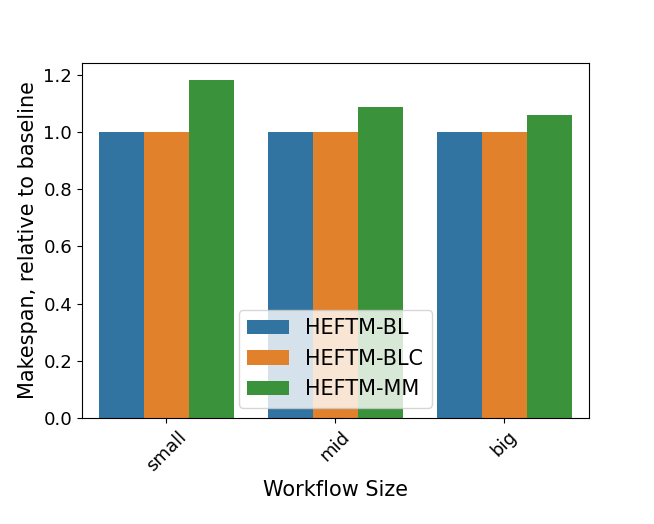
\includegraphics[width=0.495\columnwidth] {images/ms-relative-3groups}
        \caption{Relative (excess) makespan of \heftbl, \heftblc and \heftmm for different . Smaller is better.}
       \label{fig:excess-ms}
        \vspace{-0.3cm}
    \end{figure}
    \subsubsection{Memory usage}
    Minimizing memory usage is an interesting measure of the quality of the solution produced by a heuristic.
    We studied the average peak memory consumption in our cluster.
    We looked at the maximum memory usage on each processor during a task execution, and averaged it over all processors
    in the execution environment.

    The results adhere to the intuition: \heftmm produces consistently smaller memory usage among all the heuristics.
    So, for small workflows, the average memory occupation by \heftbl and \heftblc is $11.8$\% and $11.7$\%, respectively,
    while \heftmm manged to occupy $10.2$\% of memories.
    For middle-sized workflows, \heftbl and \heftblc occupied $27.8$\% and $28.2$\%, respectively, while \heftmm occupied
    $21$\%.
    For the big workflows, \heftmm occupied $20.9$\% against $33.7$\% by \heftbl and $27.6$\% by \heftblc.
    Interestingly, for big workflows, \heftmm occupied on average even a little less that for the middle-sized ones.
    This means that the bound of exploiting parallelization has been achieved for workflows around the size of middle-sized ones,
    and for the big workflows, the makespan is not improved by ``spreading'' the workflow more.

    \subsubsection{Impact of cluster size}
    On a cluster with only $18$ processors ($3$ of each kind), the baseline makes more failures: from $43.8$\%  (small workflows)
    to $77.8$\% (mid-sized) and $88.9$\% (big workflows).
    At the same time, each heuristic is unable to schedule one big workflow and one middle-sized one.
    On the workflows that they are able to schedule, \heftbl and \heftblc produce makespans that are $<1$\% bigger than
    those of the baseline on small and middle-sized workflows.
    On the big workflows, they produce makespans that are $3.5$\% and $2.3$\% bigger respectively.
    The performance of \heftmm improves more with workflow size: it goes from producing $16$\% bigger makespans on small
    workflows, to $8$\% on middle-sized ones, to $7$\% on big workflows.

   Like in the normal cluster, \heftmm again consistently shows smaller peak memory usage in the cluster.
    It utilizes on average $15$\% of memory on small workflows ($17.7$\% for \heftbl and \heftblc),
    $31$\% on middle-sied workflows ($45.2$\% and $44.9$\% on \heftbl and \heftblc, respectively),
    and $34$\% on big workflows ($50.1$\% and $50.2$\% for \heftbl and \heftblc).

    \subsubsection{Impact of cluster composition}
    On the {\em fat-and-thin} cluster, the baseline produces $60$\% invalid results on small workflows, $83.3$\% on
    middle-sized and $88.9$\% on big workflows, and therefore performs worse than on the normal cluster.

    The relative makespans are $14-29$\% worse for small workflows, $22-40$\% worse on middle-sized workflows and $16-35$\%
    on big workflows.
    \wrt failures, all heuristics again manage to schedule all workflows.
    \subsubsection{Behavior of workflow types when scaling workflow size}
    \subsubsection{Running times}
    The geometric means of runtimes of all heuristics on small workflows lie between $0.9$ and $2.2$ seconds.
    For middle-sized workflows, the runtimes for \heftbl and \heftblc are close to $2$ minutes, while \heftmm
    takes $5.1$ minutes.
    For the big workflows, again, \heftbl and \heftblc show a better runtime ($5$ and $5.4$ minutes, respectively).
    \heftmm takes $13.9$ minutes on average.
    \subsubsection{Summary}

    \section{Conclusion  \skug{Full: 0, Polished: 0}}

    \bibliographystyle{apalike}
    \bibliography{references}

\end{document}
